\documentclass{sigplanconf}[10pt] % <<<

% Keep fontenc and inputenc them in this order.
\usepackage[T1]{fontenc}
\usepackage[latin1]{inputenc}

\usepackage{amsmath}
\usepackage{amssymb}
\usepackage{graphics}
\usepackage{microtype}  % do not remove
\usepackage{proof}
\usepackage{pygmentize}
\usepackage{rgalg}
\usepackage{tikz}
\usepackage{xcolor}
\usepackage{xspace}

\usepackage{tikz}
\usetikzlibrary{arrows,positioning,fit,backgrounds,shadows,calc}

\usepackage[colorlinks]{hyperref} % keep it last to avoid some warnings

\RecustomVerbatimEnvironment{Verbatim}{BVerbatim}{}
\definecolor{darkred}{rgb}{0.4,0,0}
\definecolor{darkblue}{rgb}{0,0,0.4}
\definecolor{verylightgray}{rgb}{0.9,0.9,0.9}
\definecolor{lightblue}{rgb}{0,0,0.9}
% comment the next line for printing
\hypersetup{colorlinks,linkcolor=darkblue,citecolor=darkblue,urlcolor=darkblue}
\hypersetup{
  pdftitle={Runtime Checking with Register Automata},
  pdfauthor={Radu Grigore and Dino Distefano and Rasmus Lechedahl Petersen}}

\title{Runtime Checking with Register Automata}
%\authorinfo{Authors info whitheld for double-blind submission}
\authorinfo{Radu Grigore}
           {Queen Mary University of London}
           {rgrig@eecs.qmul.ac.uk}
\authorinfo{Dino Distefano}
           {Queen Mary University of London}
           {ddino@eecs.qmul.ac.uk}

\authorinfo{Rasmus Lerchedahl Petersen}
           {Microsoft Research}
           {rusmus@eecs.qmul.ac.uk}

\renewcommand{\sectionautorefname}{Section}
\renewcommand{\subsectionautorefname}{\sectionautorefname}

\newcommand{\noterg}[2]{\textcolor{gray}{[\textcolor{red}{#1}: #2]}}
%\renewcommand{\note}[2]{}
\newcommand{\rg}[1]{\noterg{rg}{#1}}
\newcommand{\rlp}[1]{\noterg{rlp}{#1}}
\newcommand{\dd}[1]{\noterg{dd}{#1}}
\newcommand{\dinocomment}[1]{\dd{#1}}

\newcommand{\B}{\ensuremath{\mathbb{B}}}
\newcommand{\N}{\ensuremath{\mathbb{N}}}
\newcommand{\delimitVerbatim}{\par\nobreak\smallskip\noindent}
\newcommand{\error}{\ensuremath{\textcolor{darkred}{\mathtt{error}}}\xspace}
\newcommand{\eval}[1]{[[#1]]}
\newcommand{\pattern}[1]{\ensuremath{\mathtt{\underline{#1}}}}
\newcommand{\pmap}{\rightharpoonup}
\newcommand{\set}[1]{\ensuremath{\mathsf{#1}}}
\newcommand{\start}{\ensuremath{\mathtt{start}}\xspace}
\newcommand{\verbline}[2][]{\[\text{\Verb@#2@}#1\]}

\newcommand{\eqquote}[2]{{%
  \refstepcounter{equation}\label{#2}%
  \setbox0=\vbox{\advance\hsize by-3\parindent\noindent\em#1}%
  \newdimen\x\x=\ht0 \advance\x by\dp0%
  \setbox1=\vbox to\x{\vss\hbox{(\arabic{equation})}\vss}%
  \leavevmode\\[1ex]%
  \hbox to\hsize{\hskip 1.5\parindent\box0\hfil\box1}%
  \\[1ex]}}

\newtheorem{definition}{Definition}
\newtheorem{example}{Example}
\newtheorem{notation}{Notation}

% Comment these in the final version.
\overfullrule=5pt
\showboxdepth=10
\showboxbreadth=30
% >>>
\begin{document}
\maketitle

\begin{abstract} % <<<
We introduce a new technique for checking temporal safety properties of Java programs.
Our approach is based on a new specification language for an extended class of {\em register automata} able to express complex properties of systems involving multiple interacting objects.
The specifications are then used to instrument Java byte-code so that their violations can be automatically detected at run-time.
We have validated our technique by checking several safety properties on large open source projects.
\end{abstract}

% >>>
\section{Introduction} % <<<

Interaction of objects is at the core of the object-oriented paradigm.
Programmers often have an informal and global understanding of how objects relate.
Consider for example Java collections.
A typical property one would want to state is:
\eqquote{If one iterator modifies its collection, then other existing iterators of the same collection become invalid, which means they cannot be used further.}{q:concur-it}
The formalization of the above constraint is non-trivial since it needs to keep track of {\em several objects} (at least two iterators, and one collection) and their {\em interaction} over time.

In this paper we define TOPL (Temporal Object-oriented Property Language), a language for specifying temporal safety properties of Java programs.
Similar formalisms used for runtime checking of Java programs include typestates~\cite{dblp:journals/scp/harel87} and tracematches~\cite{dblp:conf/oopsla/allanachklmsst05}.
Unlike those, TOPL is based on an automata formalism designed for {\em infinite alphabets}~\cite{dblp:conf/csl/segoufin06}.
In the context of program analysis the alphabet is the set of program values.
This set is infinite since there is no bound on the number of instantiations.
There are several such automata formalisms;
TOPL is an extension of register automata~\cite{dblp:journals/tcs/kaminskif94}.
%For standard finite-state automata, nondeterminism does not increase expressivity;
%with infinite alphabets, nondeterminism does increase expressivity.
For standard finite-state automata, nondeterminism does not increase expressivity;
however combining  infinite alphabets and nondeterminism gives strictly more expressive automata. 
Runtime checkers based on typestates~\cite{arnold:2008}, tracematches, or LTL~\cite{dblp:conf/oopsla/chenr07} are essentially deterministic, for speed.
We chose to give TOPL nondeterministic semantics.

We also introduce a technique for automatic run-time checking of TOPL properties.
Every iterator and every collection in \texttt{java.util} contains checks concerning the example property~\eqref{q:concur-it}.
It is impossible to turn off these checks, even if one has a proof that a certain program correctly uses the library.
Because these checks are always active, their overhead must be very low.
As a result, when a check fails, the user does not see an error trace.
Also, such checks are difficult to write and to maintain.
Other libraries document such temporal constraints only in comments.
With TOPL, the programmer describes the property in one place.
Then the TOPL compiler inserts appropriate checks into Java bytecode.
The execution is monitored and violations are reported as traces of events.
The programmer tunes the overhead by choosing how many objects to track, for how long to remember past events, and a few other parameters.
For example, during testing they could allow for a very high overhead, and they could chose to deploy the bytecode without any inserted check.

\rg{Should these sentences be shorter?}
In summary, the contributions of this paper are:
\begin{itemize}
\item We define the TOPL specification language, which is tailored to express properties involving object interactions over time in a way that is familiar to Java programmers.
\item We give precise formal semantics for the TOPL, making it suitable for program analysis, both static and dynamic.
\item We describe the relation between TOPL's semantic model and register automata. \dd{We need to add Rasmus' encoding}
\item We introduce a technique to automatically check at run-time violations of TOPL properties in Java programs.

\item We discuss the implementation of our technique.
\item We report the results of using our tool on large open-source projects. The results are encouraging: we have found
violations of properties, and we have observed an acceptable runtime overhead. 
\end{itemize}

\rg{Only update this at the very end.}
The paper is organized as follows.
In Section~\ref{sec:examples} we start with few motivating examples.
Section~\ref{sec:syntax} gives  TOPL's syntax  and semantics.
Section~\ref{sec:dynamic} explores the use of TOPL for run-time checking of and presents experimental results.
Section~\ref{sec:related} discusses related work.
Finally, Section~\ref{sec:conclusions} concludes the paper and describes our plans for future work.

% >>>
\section{TOPL by Examples} \label{sec:examples} % <<<

In this section we introduce TOPL in an informal way by means of examples.

\subsection{Iterators Step by Step} \label{sec:examples.steps} % <<<

The last statement in \autoref{fig:first.java} violates the property of the introduction, therefore throwing an exception.
There are two iterators on the same collection, one of them modifies the collection, and this invalidates the other iterator.
Such properties are often explained using diagrams that are sometimes precise, but not expressive enough~\cite{dblp:journals/scp/FieldGRY05,dblp:conf/issta/FinkYDRG06} or sometimes expressive, but imprecise~\cite{dblp:conf/oopsla/bierhoffa07,dblp:conf/oopsla/naeeml08,dblp:conf/sigsoft/boddenlh08,dblp:conf/ecoop/bierhoffba09}.
\autoref{fig:first.topl} (left)  captures precisely a temporal property involving three interacting objects.
On the right hand side  the same property is described in TOPL's textual form of TOPL isomorphic to the diagram.

In a TOPL property, vertices have identifiers (\texttt{start}, \texttt{one}, \texttt{two}, \dots);
transitions have labels ($\pattern I:=\pattern C.\mathtt{iterator}()$, \dots).
There are two special vertices: \start, from where the execution begins; and \error, where the execution ends.
Labels resemble the shape of statements that enable the corresponding transition.

\begin{figure}[t] % first example <<<
\begin{Verbatim}[commandchars=\\\{\}]
\PY{k+kn}{import} \PY{n+nn}{java.util.*}\PY{o}{;}
\PY{k+kd}{public} \PY{k+kd}{class} \PY{n+nc}{IncorrectIteratorUse} \PY{o}{\PYZob{}}
  \PY{k+kd}{public} \PY{k+kd}{static} \PY{k+kt}{void} \PY{n+nf}{main}\PY{o}{(}\PY{n}{String}\PY{o}{[}\PY{o}{]} \PY{n}{args}\PY{o}{)} \PY{o}{\PYZob{}}
    \PY{n}{List}\PY{o}{<}\PY{n}{Integer}\PY{o}{>} \PY{n}{c} \PY{o}{=} \PY{k}{new} \PY{n}{ArrayList}\PY{o}{<}\PY{n}{Integer}\PY{o}{>}\PY{o}{(}\PY{o}{)}\PY{o}{;}
    \PY{n}{c}\PY{o}{.}\PY{n+na}{add}\PY{o}{(}\PY{l+m+mi}{1}\PY{o}{)}\PY{o}{;} \PY{n}{c}\PY{o}{.}\PY{n+na}{add}\PY{o}{(}\PY{l+m+mi}{2}\PY{o}{)}\PY{o}{;}
    \PY{n}{Iterator}\PY{o}{<}\PY{n}{Integer}\PY{o}{>} \PY{n}{i} \PY{o}{=} \PY{n}{c}\PY{o}{.}\PY{n+na}{iterator}\PY{o}{(}\PY{o}{)}\PY{o}{;}
    \PY{n}{Iterator}\PY{o}{<}\PY{n}{Integer}\PY{o}{>} \PY{n}{j} \PY{o}{=} \PY{n}{c}\PY{o}{.}\PY{n+na}{iterator}\PY{o}{(}\PY{o}{)}\PY{o}{;}
    \PY{n}{i}\PY{o}{.}\PY{n+na}{next}\PY{o}{(}\PY{o}{)}\PY{o}{;} \PY{n}{i}\PY{o}{.}\PY{n+na}{remove}\PY{o}{(}\PY{o}{)}\PY{o}{;} \PY{n}{j}\PY{o}{.}\PY{n+na}{next}\PY{o}{(}\PY{o}{)}\PY{o}{;}
  \PY{o}{\PYZcb{}}
\PY{o}{\PYZcb{}}
\end{Verbatim}

\caption{A first example: Java code}
\label{fig:first.java}
\end{figure}
%
\begin{figure}[t]
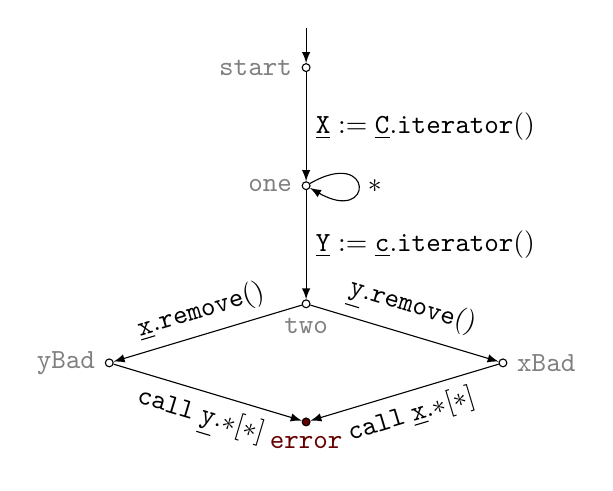
\begin{tikzpicture}
  \def\x{2.5}
  \def\y{1.5}
  \tikzset{vertex/.style={draw,circle,inner sep=1pt}}
  \tikzset{transition/.style={->,>=latex}}
  \tikzset{every label/.style={gray}}
  \node[vertex] (start) at (0,0) [label=left:\texttt{start}] {};
  \node[vertex] (one) at (0,-1*\y) [label=left:\texttt{one}] {};
  \node[vertex] (two) at (0,-2*\y) [label=below:\texttt{two}] {};
  \node[vertex] (xBad) at (1*\x,-2.5*\y) [label=right:\texttt{xBad}] {};
  \node[vertex] (yBad) at (-1*\x,-2.5*\y) [label=left:\texttt{yBad}] {};
  \node[vertex,fill=darkred] (error) at (0,-3*\y) [label=below:\textcolor{darkred}{\texttt{error}}] {};
  \draw[transition] (0,0.5)--(start);
  \draw[transition] (start)--node[right]{$\pattern X:=\pattern C.\mathtt{iterator}()$} (one);
  \draw[transition] (one) .. controls +(30:1cm) and +(-30:1cm) .. node[right]{$*$} (one);
  \draw[transition] (one)--node[right]{$\pattern Y:=\pattern c.\mathtt{iterator}()$} (two);
  \draw[transition] (two) -- node[sloped,above]{$\pattern y.\mathtt{remove}()$} (xBad);
  \draw[transition] (two)--node[sloped,above]{$\pattern x.\mathtt{remove}()$} (yBad);
  \draw[transition] (xBad)--node[sloped,below]{$\mathtt{call}\;\pattern x.{*}[*]$} (error);
  \draw[transition] (yBad)--node[sloped,below]{$\mathtt{call}\;\pattern y.{*}[*]$} (error);
\end{tikzpicture}
%\\[2ex]
\begin{Verbatim}[commandchars=\\\{\}]
property InvalidateOtherIterators
  using prefix java.util.Collection
  using prefix java.util.Iterator
  start -> one:  \pattern{X} := \pattern{C}.iterator()
  one -> one:    *
  one -> two:    \pattern{Y} := \pattern{c}.iterator()
  two -> yBad:   \pattern{x}.remove()
  two -> xBad:   \pattern{y}.remove()
  yBad -> error: call \pattern{y}.*[*]
  xBad -> error: call \pattern{x}.*[*]
\end{Verbatim}
\caption{Property {\tt InvalidateOtherIterators} in diagram (left) and textual form (right).
}
\label{fig:first.topl}
\end{figure}
%
\begin{figure}[t]
{\def\s#1{\text{\Verb@#1@}}
 \def\m#1{\PY{n+na}{#1}}
 \def\t#1{\mathtt{#1}}
\begin{align*}
&\{\;(\start,[])\;\} \\
&\s{Iterator<Integer> i = c.\m{iterator}();}  \\
&\text{//assume {\tt c} holds $1$, and {\tt i} holds $2$ } \\
& \begin{aligned}
  \{\;&(\start,[]),\
      &(\t{one},[c:1,x:2])\;\}
  \end{aligned}\\
&\s{Iterator<Integer> j = c.\m{iterator}();}  \\
&\text{//assume {\tt j} holds $3$} \\
& \begin{aligned}
  \{\;&(\start,[]),\
      &(\t{one},[c:1,x:2]),\
      &(\t{one},[c:1,x:3]),\
      &(\t{two},[c:1,x:2,y:3])\;\}
  \end{aligned}\\
&\s{i.\m{next}();} \\
& \begin{aligned}
  \{\;&(\start,[]),\
      &(\t{one},[c:1,x:2]),\
      &(\t{one},[c:1,x:3]),\
      &(\t{two},[c:1,x:2,y:3])\;\}
  \end{aligned}\\
&\s{i.\m{remove}();} \\
& \begin{aligned}
  \{\;&(\start,[]),\
      &(\t{one},[c:1,x:2]),\
      &(\t{one},[c:1,x:3]),\
      &(\t{yBad},[c:1,x:2,y:3])\;\}
  \end{aligned}\\
&\s{j.\m{next}()} \\
& \begin{aligned}
  \{\;&(\start,[]),\
      &(\t{one},[c:1,x:2]),\
      &(\t{one},[c:1,x:3]),\
      &(\error,[c:1,x:2,y:3])\;\}
  \end{aligned}\\
\end{align*}}
\caption{Running trace of {\tt InvalidateOtherIterators}. Lines \{in curly brackets\} describe automaton's states;
lines in \texttt{monotype} show executing statements;
// are comments.}
\label{fig:first.steps}
\end{figure} % >>>
\autoref{fig:first.steps} shows an execution of the program and of an automaton for the property \texttt{InvalidateOtherIterators}.
At a given moment, the automaton has a set of active states.
A state is a pair of a vertex and a store.
The store is a memory that holds (automaton) variables.
Technically, it is a finite partial map from variables to values.
We write $[k_1:v_1,k_2:v_2]$ for the finite partial map that maps key~$k_1$ to value~$v_1$, and key~$k_2$ to value~$v_2$.
The empty map is denoted by~$[]$.

The automaton has variables $x$,~$y$, and~$c$.
At vertex \texttt{one} the variables $x$~and~$c$ are initialized;
at \texttt{two} the variables $x$,~$y$, and~$c$ are initialized.
At vertex \texttt{one} $x$~is an iterator for a collection~$c$, and
at \texttt{two}, $x$~and~$y$ are both two iterators for the same collection~$c$.
Notice that~\Verb@c@ is a program variable whereas~$c$ is an automaton variable.
The same name was chosen because the two variables always hold the same value in this example.
In general, however, program variables and automaton variables live in different name-spaces, and may hold different values.

To avoid confusion, program variables are typeset in \Verb@monotype@ (\Verb@c@,~\Verb@i@,~\Verb@j@).
Automaton variables are typeset in \textit{italics} ($c$,~$x$,~$y$) and do \emph{not} appear in the property.
Instead, automaton variable \emph{patterns} appear in the property, and they are typeset in \texttt{\underline{underlined monotype}} (\pattern c,~\pattern C, \pattern x, \pattern X, \pattern y,~\pattern Y).
The interaction between patterns and automatons' memory is as follows: uppercase patterns write to the automaton memory, and lowercase patterns read from the automaton memory and act as a guard on the transition.

\paragraph{Step~1.}

Initially, only the state $(\start,[])$ is active.
The outgoing transition of vertex \start is labeled by $\pattern X:=\pattern{C}.\mathtt{iterator}()$ and the first executed statement is \verbline[.]{i = c.\PY{n+na}{iterator}()}
A method call matches a label when
\begin{itemize}
\item[(a)] the called method matches the method pattern, and
\item[(b)] the program values match their corresponding patterns.
\end{itemize}
By definition, any value matches an Uppercase pattern.
Here, the values of \Verb@i@~and~\Verb@c@ trivially match the patterns \pattern X~and~\pattern C.
The method itself also matches the method pattern.
For simplicity, we ignore argument types and identify Java methods only by their fully qualified name and their arity.
The called method \texttt{iterator} is in the class \texttt{ArrayList} and has arity~$1$.
We identify it as follows.
\verbline{java.lang.ArrayList.iterator[1]}
Without \texttt{using prefix} directives, the method pattern would be \Verb@iterator[1]@.
With the directives, however, the pattern is the following.
\begin{align*}
&\text{\Verb@java.util.Collection.iterator[1]@} \\
&\text{\Verb@java.util.Iterator.iterator[1]@}
\end{align*}
It means that these two methods \emph{and} all those that override them match.
Here, \texttt{ArrayList} implements \texttt{Collection}.

All conditions are met to enable the transition from \start to \texttt{one}.
When the transition is performed the values that matched \pattern X~and~\pattern C are written in the automaton variables $x$~and~$c$.
For concreteness, let us assume these values are $1$~and~$2$.
After the transition is performed, the state $(\mathtt{one},[c:1,x:2])$ is active.
The state $(\start,[])$ remains active because the implicit transition \verbline{start -> start: *} is also enabled and performed.

\paragraph{Step~2.}
For the second step, the statement to be executed is \verbline[.]{j = c.\PY{n+na}{iterator}()}
Now we need to consider, in turn, the two active states \[\{(\start,[])\quad\text{and}\quad(\texttt{one},[c:1,x:2])\}\]
For $(\start,[])$ the same reasoning as for step 1 holds, so the states $(\start,[])$ and $(\mathtt{one},[c:1,x:3])$ are active after step~2.
Note that now the automaton variable~$x$ remembers the value of the program variable~{\tt j}.
For $(\texttt{one},[c:1,x:2])$ we look at the transitions outgoing from vertex {\tt one}.
\begin{align*}
&\text{\Verb@one -> one: *@} \quad \mbox{ and } \quad
\text{\Verb@one -> two: \pattern Y := \pattern c.iterator()@}
\end{align*}
The first transitions is always enabled, and performing it keeps states with vertex \texttt{one} active.
The second transitions has two patterns, \pattern Y~and~\pattern c.
The uppercase pattern~\pattern Y always matches, whereas
pattern \pattern c matches only the value held by the automaton variable~$c$.
In this case, $c$ was set in the previous step to the value of the program variable~\texttt{c}.
Therefore, the transition from~\Verb@one@ to~\Verb@two@ is performed and the state $(\mathtt{two},[c:1,x:2,y:3])$ is activated.

\paragraph{Step~3.}

The third step involves the statement
\[\text{\Verb+\PY{n}{i}\PY{o}{.}\PY{n+na}{next}\PY{o}{(}\PY{o}{)}\PY{o}{;}+}\]
which matches no label of outgoing transitions of the currently active vertices (that is, \start, {\tt one}, and {\tt  two}).
Therefore, although the program proceeds, the set of active states of the automaton remains unchanged.

\paragraph{Step~4.}

In the fourth step, the transition $\texttt{two}\to\texttt{yBad}$ is performed.
Notice that the pattern $\pattern{x}.\mathtt{remove}()$ does not have a left-hand side, which simply means that the returned value is irrelevant for this transition.
The states corresponding to vertices \start and {\tt one} remain unchanged, because their outgoing transitions are disabled.
However,  the outgoing transition of state {\tt two} is enabled, and therefore {\tt yBad} becomes active.

\paragraph{Step~5.}

For the fifth and final step, the statement to be executed is \verbline[.]{j.\PY{n+na}{next}()}
The label of the outgoing transition  \[\mathtt{call}\;\pattern{y}.{*}[*]\] of the active state $(\texttt{yBad},[c:1,x:2,y:3]),$
has two distinguishing features: the~$*$ as a method name and the tag \texttt{call}.
As before, in order to match the method name, the prefixes
\Verb@java.util.Collection.*[*]@ and \Verb@java.util.Iterator.*[*]@
are prepended.
Then the $*$s are expanded, taking into account the \texttt{CLASSPATH}.
The expansion \Verb@java.util.Iterator.next@ is overridden by the method that is actually called and therefore 
we have a match.

The tag {\tt call} is used when we want the automaton to take a transition precisely at call-time of a method invocation.
The automaton expresses that a call to one of {\tt j}'s methods while vertex \texttt{yBad} is active constitutes an error.
Notice that this is different from a label like $\pattern X:=\pattern C.\mathtt{iterator}()$ which may match only after the return value is known.

\medskip
The execution we stepped through reaches the \error vertex, so we conclude that the property is violated.
Notice that in order to find a counterexample we need to keep track of the relation between several objects, in particular that iterators {\tt i} and {\tt j} are for the same collection {\tt c}.

% >>>
\subsection{Heap Shape and Values Sensitive Properties}  % <<<
One interesting kind of properties for object-oriented programs is the ability to reason about the shape of the heap composed by the allocated objects.
The following TOPL's properties test the shape of a linked list and reports an error if it is cyclic or it has the pan-handle shape (i.e., there is a lasso at some point).
%
\delimitVerbatim
\begin{Verbatim}[commandchars=\\\{\}]
property ListNotCyclic
   start -> a: \pattern{X} := *.getList()
   a -> a:     \pattern{X} := x.next()
   a -> b:     \pattern{Y} := x.next()
   b -> b:     \pattern{Y} := y.next()
   b -> error: x := y.next()
   a -> error: x := x.next()
\end{Verbatim}
\delimitVerbatim
The idea is that this property will bind the automaton variable $x$ with any possible object in the list, and the $y$ with any possible successors (via the next field) of the current binding of $x$.
Therefore, if there is a lasso, in the list, this will be detected when a new biding of $y$ via a \texttt{b -> b} becomes equal to the binding of $x$.
The transition \texttt{a ->error} detect the case where there is an object pointing to itself.


The following property detects when a dictionary overwrite one of its bindings.
\delimitVerbatim
\begin{Verbatim}[commandchars=\\\{\}]
 property BadDictionary
   message "the dictionary overwrite its bindings"
   prefix <Dictionary>
   start -> written:   \pattern{D}.put(\pattern{K}, \pattern{V})
   written -> written: d.put(k, \pattern{V})
   written -> error:   !v := d.get(k)
\end{Verbatim}
\delimitVerbatim
The overwrite is detected by the guard which checks if the value associated with a key $k$ is the same as the original binding recorded in the automaton variable $v$.

% >>>
% >>>
\section{TOPL Syntax and Semantics} % <<<
\label{sec:syntax}
Syntactically, a TOPL property has a name, a set of \texttt{using} directives, and a set of transitions.
Each transition is a labelled arc (directed edge) with a source and a target vertex identified by their name.
Labels look like method calls.
Each label has a method pattern that is used to identify the set of methods to which the label refers.
In the simple case, a method pattern consists of a string pattern for the name of the method and an integer that specifies the method arity.
(For simplicity, TOPL does not use the static types of arguments to distinguish between overloaded methods.)
The more interesting case is when there are value patterns for each argument and perhaps even for the result.
Transitions should typically be tagged with \texttt{call} or \texttt{return} to specify exactly at what time they should be performed.
Name patterns are POSIX globs and match method names.

\paragraph{On the Value Patterns mechanism.}
For each automaton variable \Verb@v@ there are three associated patterns.
The uppercase pattern \Verb@V@ matches any value and writes it in the automaton variable \Verb@v@.
The lowercase pattern \Verb@v@ reads the value of the automaton variable \Verb@v@ and only matches that value.
The negated lowercase pattern \Verb@!v@ reads the value of the automaton variable \Verb@v@ and only matches different values.
A Java literal acts as a pattern that matches only the value it denotes.
A wildcard~* pattern matches any value.

\smallskip
A TOPL property is \emph{well-formed} when it satisfies the following two conditions:
{\em (i)} labels must contain uppercase value patterns at most once; {\em (ii)}
any use of a lowercase patterns must be preceded by a use of the corresponding uppercase pattern on all paths from \start  (i.e., automaton variables must be written before being read).
From now on we assume TOPL properties to be well-formed.

\subsection{Semantics}\label{sec:semantics} % <<<
We model the semantics of programs and automata as sets of event traces.
We say that a program \emph{violates} a property when their sets of traces intersect.
In other words, properties encode bad executions, rather than good executions.

\subsubsection{TOPL execution automata.}
\newcommand{\World}{ExecState}

Each TOPL's property when considered in conjunction with the set of traces defining the semantics of the program, gives rise to an automaton defined over the labeled multigraph  on $\set{Vertex}$ and $\set{Arc}$.
This automaton represents the semantics of the property interpreted over the program.
$\set{Vertex}$ is the set of vertices mentioned as endpoints of the arcs and $\set{Arc}$ is the set of labeled arcs mentioned in transitions.
The automaton has two special vertices, {\tt start} and {\tt error},  i.e., the initial and accepting vertex respectively.

We assume a countable set \set{Value} of values and a countable set $\set{Variable}$ of automaton variables.
Let stores be finite partial maps with finite domain.
\[
\set{Store} = \set{Variable} \pmap_{\mathit{fin}} \set{Value}
\]
Moreover we assume a countable set \set{Event} of events with known arity.
Each event~$e$ is of the form $(t_e,[0{:} v_0,\dots, 1{:}v_n])$.
The component $t_e$ is a tag, e.g., {\em call} or {\em return}, while the second component is an array of values.
Within guards and actions we write $tag(e)$ for the tag, and $e[i]$ for the $i$th value of the array.
%
\begin{definition}[TOPL execution automaton]
Given a TOPL property $(\set{Vertex},\set{Arc})$ and a set of program traces $\set{Trace}$, a {\em TOPL execution automaton} $\Xi$ is a tuple
$(\set{State}, \to , \set{Init}, \set{Error})$ where
\begin{itemize}
\item $\set{\World} \subseteq (\set{Vertex}\times \set{Store})\times\set{Trace}$ is a set of {\em execution states}.
\item $\to \subseteq \set{\World} \times \set{\World}$ is a set of {\em execution transitions}
\item $\set{Init}= \{ (\texttt{start}, [], \tau) \mid \tau \in \set{Trace} \}$ is the set of initial execution states;
\item $\set{Error} \subseteq \{ (\texttt{error}, \sigma, \tau) \mid \sigma \in \set{Store},  \ \tau \in \set{Trace} \}$ is the set of accepting (error) execution states.
\end{itemize}
\end{definition}
A state of the automaton is given by specifying the vertex in the graph as well as the value of defined automaton variables and a trace of events to be observed.
The reader may wonder why execution states need to contain traces.
The reason is that each label in $\set{Arc}$ carries (potentially) a list of guards and we call the length of this list, the \emph{depth} of the arc.
Since different outgoing arcs for a vertex can have different depths, we have that different target states of execution transitions may receive different events.
For example, for a trace of events $e_1 e_2 e_3\cdots$, if two outgoing transitions from the same state have depth 2 and 5 rispectively, then the end state of the first transition will see $e_3$, while the end state of the second transition $e_6$.

In order to define the transition relation $\to$ we need to define two auxiliary concepts.
When observing a trace, the effect of actions in an arc label on a store  is given by the function
\[
   A : \set{Store} \times \set{Trace} \times \set{Label} \to \set{Store}_\bot
\] and defined as
\[
\begin{array}{l}
\begin{array}{lcl}
A(\sigma,\epsilon,l) & = & \bot
\\[2ex]
A(\sigma,e,(g,a)) & = & \left\{\begin{array}{ll}
     a(e,\sigma) & \mbox{if $g(e,\sigma)$}
     \\[1ex]
     \bot & \mbox{otherwise}
     \end{array}
     \right.
\\[5ex]
A(\sigma,e\cdot \tau,(g,a)\cdot l) & = & \left\{\begin{array}{ll}
     A(\sigma',\tau,l) & \mbox{if $|\tau|{=}|l|{>}0$ and }
     \\
& \mbox{$A(\sigma,e,(g,a)){=}\sigma'$}
     \\[1ex]
     \bot & \mbox{otherwise}
     \end{array}
     \right.
\end{array}
\end{array}\]
In this definition, the effect of a list of actions $l$ on an empty trace $\epsilon$ gives the undefined value.
If the event $e$ passes the guard $g$ in the store $\sigma$, the corresponding action $a$ is performed on that event and therefore updating the store $\sigma$.

With $A$ we can define the predicates $enabled$ testing whether a transition is enabled in a store when observing a trace, and a predicate $Enabled$ testing if there exists an enabled transition starting from an execution state:
\begin{eqnarray*}
enabled(\sigma,\tau,l) & \Leftrightarrow & A(\sigma,\tau,l) \neq \bot
\\
Enabled(x,\sigma,\tau) & \Leftrightarrow  & \bigvee \{ enabled(\sigma,\tau,l) \mid x \to x' : l \}
\end{eqnarray*}
Notice that, according to the definition of $enabled(\sigma,\tau,l)$, and in turn of the function $A$, for a transition to be enabled, all the guards along its list have to evaluate to true.
Evaluating a guard along the transition consumes an event |  therefore | to see if a transition is enabled we have to examine $|l|$ events.

The transition relation $s \to s'$ is defined by the following rules.
\[
\begin{array}{ll}
\text{(Step)}  &
\infer[x_1 \to x_2{:} l \mbox{ and } |l|{=}|\tau_1| ]{ (x_1,\sigma_1,\tau_1 \cdot \tau_2 ) \  \to \  (x_2, \sigma_2, \tau_2)}{A(\sigma_1,\tau_1,l)=\sigma_2}
\\[2ex]
\text{(Silent)}  &
\infer[\neg Enabled(x_1,\sigma_1,\tau_1) ]{ (x_1,\sigma_1,\tau_1) \  \to \  (x_1, \sigma_1, \tau_2)}{ \tau_1=e \cdot \tau_2}
\end{array}
\]
Finally, we can define the language of a TOPL execution automaton $\Xi$, as the set of traces it accepts:
\[
{\cal L}(\Xi) = \{ \tau \mid \exists \sigma' \tau', (\mathtt{start},[],\tau) \to^* (\mathtt{error},\sigma',\tau')\}
\]
${\cal L}(\Xi)$ are the traces that drive the automaton $\Xi$ from the \texttt{start} vertex (with an empty store) to the \texttt{error} vertex.

\paragraph{Silent steps.}
A peculiar aspect of the transition relation $\to$ is that if no transitions are enabled for a given state and trace of events, the automaton does not get stuck but it consumes one event without changing its state (see the  Silent Step rule).
Note that a silent step is not equivalent to a self-loop on all states, as dropping events is not allowed if there are enabled transitions.
In that case,  the enabled transitions are performed with the rule (Step) and the automaton execution state becomes $(x_2, \sigma_2,\tau_2)$, where $x_2$ is the target vertex of the arc of the transition, $\sigma_2$ is defined by the modification imposed by the function $A$ and $\tau_2$ is the leftover of the event trace before the transition after dropping $|l|$ events.
\begin{example}
Consider the automata in Fig.~\ref{fig:unmatched-example} and assume that the set of active states for the left-hand side automaton is $\{ \texttt{zero} \}$ and for the right-hand side one is $\{ \texttt{three}\}$.
Moreover, let us assume that our input trace is $\cdots e_1 e_1 e_2 \cdots$ In the left-hand side automaton, the first occurrence of the event $e_1$ enables the transition  from {\tt zero} to {\tt two}, however, the transition from {\tt zero} to {\tt one} cannot fire since the first occurrence of $e_1$ (in the trace) is followed by another $e_1$.
Consequently, after the first occurrence of $e_1$ state {\tt two} becomes active and {\tt zero} inactive.
Notice that, in the left-hand side automaton, state {\tt one} cannot be reached by the trace $e_1 e_1 e_2 $ from {\tt zero}.
On the contrary, for the right-hand side automaton, the first occurrence of $e_1$ does not enable any transition per se.
Notice that the only outgoing transition on the active state {\tt three} needs a sequence of two events to be enabled.
Hence, we need to consider the sequence $e_1e_1$.
The latter does not enable any transition either.
Therefore, according to our semantics,  the first occurrence of $e_1$ is consumed silently and the set of active states (i.e., $\{ \texttt{three} \}$) remains unchanged.
At this point, the second occurrence of $e_1$ is considered, and since it is followed by $e_2$, the transition from {\tt three} to {\tt four} becomes enabled.
Events $e_1e_2$ are consumed, {\tt four} becomes active and {\tt three} inactive.
\end{example}

\begin{figure}[t]
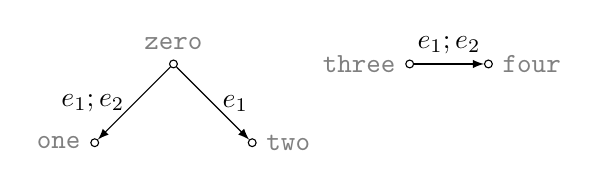
\begin{tikzpicture}
  \def\x{2.5}
  \tikzset{vertex/.style={draw,circle,inner sep=1pt}}
  \tikzset{transition/.style={->,>=latex}}
  \tikzset{every label/.style={gray}}
  \node[vertex] (zero) at (0,0) [label=above:\texttt{zero}] {};
  \node[vertex] (one) at (-1,-1) [label=left:\texttt{one}] {};
  \node[vertex] (two) at (1,-1) [label=right:\texttt{two}] {};

  \node[vertex] (three) at (3,0) [label=left:\texttt{three}] {};
  \node[vertex] (four) at (4,0) [label=right:\texttt{four}] {};

  \draw[transition] (zero)--node[left]{$ e_1;e_2$} (one);
  \draw[transition] (zero)--node[right]{$e_1$} (two);

  \draw[transition] (three)--node[above]{$e_1;e_2$} (four);
\end{tikzpicture}
\caption{Example of unmatched events.}
\label{fig:unmatched-example}
\end{figure}

\subsubsection{On labels and guards.} % <<<

A label is a list of pairs $(g,a)$ of guards and actions. A  {\em general guard} is a partial function of type:
\[
\set{GenGuard} = (\set{Pattern} \times \N \times \set{Pred}) \pmap (\set{Event}\times\set{Store}) \to \B
\]
An {\em instantiated guard} is a general guard provided with instances of a pattern  name $\pattern v$,  its position $i$ in the label, and a predicate $p$ needed to test this pattern:
\[
g_{\pattern{v},i,p} : \set{Event}\times\set{Store} \to \B
\]
Given an event and a store, an instantiated guard  evaluates whether the event satisfy the guard in the store. It is defined as:
\newcommand{\sem}[1]{[ \! | #1 | \! ]}
\[
g_{\pattern{v},i,p}(e, \sigma) = p(e[i],\sigma(\pattern v))
\] The guard is true if and only if the value of $\pattern{v}$ in the automaton store
and the value of $i$-th parameter of  event $e$ (obtained from the program store) satisfy $p$.
\begin{example}
Consider the label
 $\sim \pattern {v} := \pattern {s}.gets(\pattern {k})$ to be matched with the statement
 {\tt t:=z.gets(h)}. Internally,  the label is compiled down to the sequences
\[
\pattern{call} \  \pattern{s}^0 .gets(\pattern {k}^1);  \ \pattern{ret} \ gets = \sim \pattern {v}^0
\] The upper-script stands for the position of a pattern in an expression. The statement generates the trace of events $e_1 \cdot e_2$ where
\[
 e_1=(call \ gets, [0: \sem{z}, \ 1: \sem{h}])  \ \mbox{ and }  \  e_2= (ret \ gets, [0: \sem{t}])
\]
The instantiated guard for the label are:
 $g_{\pattern{s},0,=}$, $g_{\pattern{k},1,=}$, and  $g_{\pattern{v},0, \neq}$.
Notice that the predicates we want to use to compare patterns and events' values are: equality for the element $\pattern{s}$ and $\pattern{k}$,
but inequality for \pattern{v} (because of $\sim$).
The instantiated guards, can now be evaluated with the events by taking their conjunction:
\[
 (tag(e_1)= \ call \ gets) \wedge g_{\pattern{s},0,=}(\sigma,e_1) \wedge g_{\pattern{k},1,=}(\sigma, e_1)
\] and
\[
 (tag(e_2)= ret \ gets) \wedge g_{\pattern{v},0,\neq}(\sigma,e_2).
\]
\end{example}

% >>>
% >>>
% >>>
\section{Run-time checking} \label{sec:dynamic} % <<<

In this section we describe an algorithm to check at run-time  TOPL properties on Java programs.
Figure~\ref{architecture} summarises our method.
There are two main components:
the {\em TOPL compiler} and the {\em Property Checker}.
The TOPL compiler takes as input compiled class files and a list of TOPL properties to be checked against the classes.
The compiler has two submodules: the {\em instrumenter} and the {\em automaton generator}.
The latter synthesises a Java program that precisely encodes the automata representing the TOPL properties.
The instrumenter instruments the byte code with calls to methods of the Java encoding of the automata.
During their tasks, the two submodules need to exchange information about method identifiers, therefore their operations are intertwined.
The property checker module can be seen as a general interpreter able to execute TOPL automata properties.
When compiled together with the Java encoding of the automata generated by the TOPL compiler, we obtain an executable property checker instantiated to the particular list of TOPL properties we want to check against the initial class files.
When run together with the instrumented class files, the instantiated property checker acts as a monitor that is able to detect violation of the properties of interest.

The TOPL compiler (\textsf{toplc}) is written in OCaml whereas  the TOPL checker is written in Java.

\begin{figure}[htbp]
\begin{center}
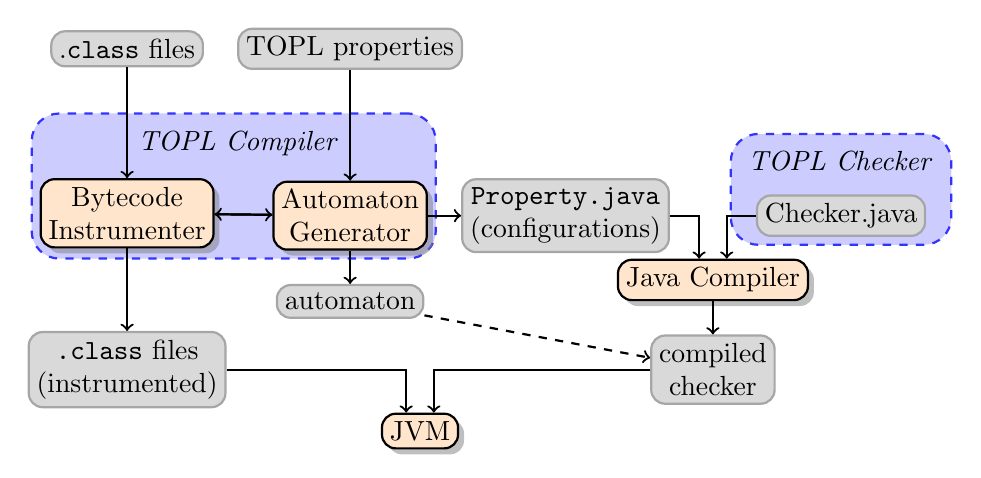
\begin{tikzpicture}[node distance=12pt, auto]
\tikzstyle{system}=[rectangle,
                                draw=blue!80,
                                fill=blue!20,
                                inner sep=0.1cm,
                                rounded corners=10pt,
                                style=dashed,thick]
\tikzstyle{program}=[rectangle,
                                  draw=black,
                                  fill=orange!20,
                                  inner sep=0.1cm,
                                  rounded corners=5pt,
                                  style=thick,
                                  drop shadow]
\tikzstyle{data}=[rectangle,
                            draw=gray!70,
                            fill=gray!30,
                            inner sep=0.1cm,
                            rounded corners=5pt,
                            style=thick]
\node[data] (classes) {{.\tt class} files};
\node[data, right=of classes] (properties) {TOPL properties};

\node[below=of classes] (classesd) {};
\node[below=of properties] (propertiesd) {};

\node[program, below=40pt of classes, align=center] (instrumenter)
  {Bytecode\\Instrumenter};
\node[program, below=40pt of properties, align=center] (genautomaton)
  {Automaton\\Generator};

\node[data, right=of genautomaton, align=center] (javaproperties)
  {{\tt Property.java}\\(configurations)};
\node[data, below=of genautomaton] (automaton) {automaton};
\node[right=of javaproperties] (javadummy) {};
\node[data, right=of javadummy] (checker) {Checker.java};
\node[program, below=of javadummy] (javac) {Java Compiler};

\node[data, below=of javac, align=center] (classproperties)
  {compiled\\checker};
\node[data, align=center] at (instrumenter |- classproperties)
  (instrclasses) {{\tt .class} files\\(instrumented)};
\node at ($(instrclasses)!.5!(classproperties)$) (classdummy) {};
\node[program, below=of classdummy] (jvm) {JVM};

\node[above=5pt] at ($(instrumenter.north)!.5!(genautomaton.north)$) (topllabel) {\emph{TOPL Compiler}};
\node[above=5pt of checker] (checkerlabel) {\emph{TOPL Checker}};
\begin{pgfonlayer}{background}
  \node[system, fit = (topllabel) (instrumenter) (genautomaton)] (TOPLC) {};
  \node[system, fit = (checker) (checkerlabel)] (CHECKER) {};
\end{pgfonlayer}

\path[thick, ->]
(classes) edge (instrumenter)

(genautomaton) edge (instrumenter)
(instrumenter) edge (genautomaton)

(properties) edge (genautomaton)
(genautomaton)  edge (javaproperties)
(javac) edge (classproperties)

(genautomaton) edge (automaton)

(instrumenter) edge (instrclasses);

\draw[thick, ->]
(instrclasses) -| ($(jvm.north)-(5pt,0)$);
\draw[thick, ->]
(classproperties) -| ($(jvm.north)+(5pt,0)$);
\draw[thick, ->]
(javaproperties)  -| ($(javac.north)-(5pt,0)$);
\draw[thick, ->]
(checker)  -| ($(javac.north)+(5pt,0)$);

\draw[thick, ->, dashed]
(automaton) -- (classproperties);
(\end{tikzpicture}

\caption{Architecture of TOPL properties' run-time checking.}
\label{architecture}
\end{center}
\end{figure}

\subsection{TOPL Compiler} % <<<

The input of the compiler is a set of properties and a set of classes and its output  is a checker and instrumented classes.
The checker is itself a Java class.
The instrumented classes have the same behaviour as the original classes but
 they are allowed to use more resources.
The compilation of TOPL properties is done by the following phases 4 phases.

\paragraph{Desugaring.}
In the first phase the parser de-sugars the TOPL properties into a simpler, intermediate form where
\begin{itemize}
\item method-name patterns are prefixed according to the \textsf{prefix} directive;
\item \textsf{call} and \textsf{return} transitions get one step, while other transitions are de-sugared into a \textsf{call} followed by a \textsf{return};
\item lowercase patterns and constant patterns are turned into guards;
\item uppercase patterns are turned into actions.
\end{itemize}
The parser builds an AST that closely follows the language for which we have formal operational semantics.

\paragraph{Static Checks.}
In the second phase, the compiler checks that the property is well-formed.
In doing so, it effectively checks that:
\begin{itemize}
\item two parallel writes to automaton variables have distinct destinations;
\item reads from automaton variables must be preceded by writes.
\end{itemize}

\paragraph{Dealing with Inheritance.}
In the third phase, the property is transformed so it explicitly identifies Java methods.
As described in Section~\ref{sec:syntax}, each transition step has a guard containing a tag component.
A \emph{tag} has a method name pattern, an arity pattern, and an event type pattern.
The latter is either \textsf{call} or \textsf{return}.
For example the tag guard ``\textsf{call *.$\langle$freeboogie.*.eval$\rangle$[2]}'' refers to all the calls to methods with two arguments whose full name matches the pattern ``\textsf{freeboogie.*.eval}'' \emph{and all the methods that override them}.
A tag guard together with a set of class signatures determine a set of program points.
Each tag guard is translated into a set of identifiers.

An \emph{observable} method is one whose name matches a pattern that appears in an \textsf{observing} directive.\dinocomment{check that observing directive have been introduced before}
Internally, each observable method in the classpath receives two integer identifiers: one for the call event and one for the return event.

At this point several properties are merged into a single property that may have multiple start vertices.
%Vertices are no longer identified by name.
The pattern of observable methods of the property is now replaced by 
a set of observable event identifiers for each vertex.

The initial property may use Java literals that are collected into an array \textsf{constants} of \textsf{Object} that is written in the file \textsf{topl/Property.java}  whereas the property is dumped into an easy-to-parse textual format, in the file \textsf{Property.text}
referring to constants by their index in the array \textsf{constants}.

\paragraph{Instrumentation.} In the last phase, 
the bytecode of each observable method is instrumented.
The first and last actions performed by the instrumented version are calls to {\sf topl.Checker.check(event)}.
Each \textsf{event} carries an identifier and an array of \textsf{Object}.
The array holds either the arguments, or the return value.

For instrumenting Java bytecode we use a fork of the library Barista~\cite{cite-barista}.
Our version of Barista handles low-level details such as relative offsets given as a count of bytes.

% >>>
\subsection{Checker} % <<<

The runtime checker of TOPL properties resides entirely in the file {\sf topl/Checker.java}.
By default, the checker logs a message when it detects a property violation. However, the action to take can be configurable and the user can choose to have an exception instead.

The main components of the checker are:
\begin{itemize}
\item a parser for the data structures used to represent properties;
\item the data structures used to represent the current state of the checker; and
\item the code that handles one incoming event.
\end{itemize}

\paragraph{Parsing and AST\null.}
The parser builds ASTs based on the content of \textsf{Property.text}.
We needs build \textsf{Property.text} since we have experienced that if we were to
 generate directly Java code that instantiates the ASTs,
 then we sometimes run over the bytecode limit on the size of methods.

\paragraph{States.}
The checker maintains a set of active states.
Each state has a queue of events to be processed.
The checker does not assume a bounded transition depth, but the compiler produces only transitions with $1$~or~$2$ steps.
If all transitions would have the same depth, then one global queue of events would suffice.

Each state also has an integer vertex identifier and a set of bindings from automaton variables to values.
Automaton variables are identified by integers; values are instances of \textsf{Object}.
Each state is produced by applying an action to another state (called the parent).
For error reporting, each state keeps track of its parent.
An active state with $\ge2$~outgoing transitions produces $\ge2$~active states for the next time step.
The new active states and their parent are likely to have similar sets of bindings.
This is why we use persistent (functional) sets for bindings; more precisely, we use treaps~\cite{treaps}.

\paragraph{Step.}
The method \textsf{topl.Checker.check(event)} is the main loop of the checker and is reported in Figure~\ref{checker.check}.
We assume the time is discrete, and advances when the program sends an event to the checker.

The checker does not do anything if it is inactive.
%The JVM (\textbf Java \textbf virtual \textbf machine) uses selected parts of the JDK during startup.
%If those parts are instrumented by the TOPL compiler, and if the TOPL checker calls back into the JDK, then the JVM crashes.
%As a workaround, the checker is inactive by default.
Ideally, \textsf{toplc} should insert bytecode that activates the checker.
Currently one has to manually insert a call to \textsf{Checker.activate}, probably as the first action of the project's \textsf{main} method.
The inactive flag is necessary to avoid recursive invocations of the checker.
\dd{Radu can you explain the algorithm in the figure?}
\begin{figure}[htbp]
\begin{center}
\begin{alg}
\^  $\proc{Check}(e)$
\=  $A := \emptyset$
\=  for each active state $s$
\+    if $\mathit{vertex}(s)$ does not observe $\mathit{id}(e)$
\+      insert $s$ into $A$
\=      continue from $3$
\-    push $e$ to the queue $\mathit{events}(s)$
\=    if $\mathit{events}(s)$ is shorter than the longest transition from $\mathit{vertex}(s)$
\+      continue from $3$
\1    $\mathit{skip}:=\mathsf{true}$
\=    for each transition $t$ outgoing from $\mathit{vertex}(s)$
\+      $\sigma := \mathit{store}(s)$,\quad $E := \mathit{events}(s)$
\=      for each step $\tau$ of $t$
\+        pop $\varepsilon$ from the queue $E$
\+        if $\proc{Guard}(\tau, \varepsilon, \sigma)$
\+          $\sigma := \proc{Action}(\tau, \varepsilon, \sigma)$
\-        else
\+          continue from 11
\2      $\mathit{skip}:=\mathsf{false}$
\=      insert state $(\mathit{target}(t), \sigma, E)$ into $A$
\=      if $\mathit{target}(t)$ is an error vertex, report the error
\=      if \textit{skip}
\+        $s' := s$
\=        insert state $s'$ with one event popped into $A$
\end{alg}
\caption{The method \textsf{topl.Checker.check(event)}.}
\label{checker.check}
\end{center}
\end{figure}

%TODO: forget states (with strategies), runtime abstraction.


\paragraph{Run-time completeness.}
\dinocomment{maybe we remove this paragraph...}
Doing concrete run-time checking is obviously unsound since only the actual runs are checked.
Our checker is also {\em incomplete}, that is:
if a run-time execution of the program leads to an error then there is no guarantee that the checker will detect the error.
The program in Figure~\ref{fig:completeness} shows that to achieve completeness any run-time checker keeping track of concrete states would need an unbounded amount of memory.
The method {\tt NeedsUnboundedMemory(int n)}
declares an array of iterators of a length depending on the external parameter {\tt n}.
 In the {\tt for} loop, the array is filled with iterators for the same collection {\tt c} and randomly some of them are exhausted by advancing till the end (inner {\tt while} loop).
Outside the {\tt for} loop, a random iterator is advanced one more time and we would get an exception if this iterator was one of those exhausted in the previous loop.
Because of the random choice of iterators, it becomes apparent that, if we were to decide at {\tt a[r.nextInt(n)].next()} whether an exception needs to be thrown or not, we would need to keep information about all the iterators.
Moreover, since their number {\tt n} is a parameter, there is no way to bound the amount of memory to keep track of this info.
\begin{figure}[htbp]
\begin{center}
\begin{Verbatim}[commandchars=\\\{\}]
\PY{k+kn}{import} \PY{n+nn}{java.util.*}\PY{o}{;}
\PY{k+kd}{public} \PY{k+kd}{class} \PY{n+nc}{Completeness} \PY{o}{\PYZob{}}
   \PY{n}{Collection} \PY{n}{c}\PY{o}{;}
   \PY{n}{Random} \PY{n}{r}\PY{o}{=}\PY{k}{new} \PY{n}{Random}\PY{o}{(}\PY{o}{)}\PY{o}{;}
   \PY{k+kd}{public} \PY{k+kt}{void} \PY{n+nf}{NeedsUnboundMemory}\PY{o}{(}\PY{k+kt}{int} \PY{n}{n}\PY{o}{)} \PY{o}{\PYZob{}}
      \PY{n}{Iterator}\PY{o}{[}\PY{o}{]} \PY{n}{a} \PY{o}{=} \PY{k}{new} \PY{n}{Iterator}\PY{o}{[}\PY{n}{n}\PY{o}{]}\PY{o}{;}
      \PY{k}{for} \PY{o}{(}\PY{k+kt}{int} \PY{n}{i}\PY{o}{=}\PY{l+m+mi}{0}\PY{o}{;} \PY{n}{i}\PY{o}{<}\PY{n}{n}\PY{o}{;} \PY{n}{i}\PY{o}{+}\PY{o}{+}\PY{o}{)} \PY{o}{\PYZob{}}
          \PY{n}{a}\PY{o}{[}\PY{n}{i}\PY{o}{]}\PY{o}{=}\PY{n}{c}\PY{o}{.}\PY{n+na}{iterator}\PY{o}{(}\PY{o}{)}\PY{o}{;}
          \PY{k}{if} \PY{o}{(}\PY{n}{r}\PY{o}{.}\PY{n+na}{nextBoolean}\PY{o}{(}\PY{o}{)}\PY{o}{)} 
	    \PY{k}{while} \PY{o}{(}\PY{n}{a}\PY{o}{[}\PY{n}{i}\PY{o}{]}\PY{o}{.}\PY{n+na}{hasNext}\PY{o}{(}\PY{o}{)}\PY{o}{)} \PY{n}{a}\PY{o}{[}\PY{n}{i}\PY{o}{]}\PY{o}{.}\PY{n+na}{next}\PY{o}{(}\PY{o}{)}\PY{o}{;}	
      \PY{o}{\PYZcb{}}\PY{o}{;}
      \PY{n}{a}\PY{o}{[}\PY{n}{r}\PY{o}{.}\PY{n+na}{nextInt}\PY{o}{(}\PY{n}{n}\PY{o}{)}\PY{o}{]}\PY{o}{.}\PY{n+na}{next}\PY{o}{(}\PY{o}{)}\PY{o}{;}
  \PY{o}{\PYZcb{}}\PY{o}{;}
\PY{o}{\PYZcb{}}
\end{Verbatim}

\caption{Counterexample to run-time completeness.}
\label{fig:completeness}
\end{center}
\end{figure}

\dinocomment{discuss about: conservative and transparent properties of an inliner}
\dinocomment{talk about our strategy}

% >>>
% >>>
\section{Experimental Results} % <<<

\rg{Move after introduction.}
\rg{Start with a section on methodology.
Explain why we don't expect to find new bugs.}

We have used the DACAPO bechmarks~\cite{dblp:conf/oopsla/dacapo} to test our tool.
We run the experiments on and Intel  Core i5 CPU  661  \@ 3.33GHz with 4GB of memory, running
 Linux 2.6.32-40 and  Java 1.6.0\_20.
To instrument the 160M of DACAPO sources and the JRE, it took  7 minutes and 4 seconds.

\begin{table*}[t]
      \centering
   \begin{tabular}{| l | r | r | r | r | }
   \hline
  Benchmark  & Original Time (Stand. Dev.) & Instrumented Time (Stand. Dev.) & Checker Memory & Failed Property
\\ \hline \hline
Tomcat 6.0.20 &  5436 (+/-141) & 7449 (+/-134) & &
\\ \hline
Benchmark 3 & & &  &
\\ \hline
Benchmark 4 & & &  &
\\ \hline
Benchmark 5 & & &  &
\\ \hline
Benchmark 6 & & &  &
\\ \hline
Benchmark 7 & & &  &
\\ \hline
Benchmark 8 & & &  &
\\ \hline
Benchmark 9 & & &  &
\\ \hline
Benchmark 10 & & &  &
\\ \hline
Benchmark 11 & & &  &
\\ \hline
Benchmark 12 & & &  &
\\ \hline
\end{tabular}
    \caption{Experimental results on the DACAPO benchmarks. The times are the average of 5 runs.}
   \label{tab:booktabs}
\end{table*}

\paragraph{Tomcat 6.0.20.}
Dacapo uses Tomcat version 6.0.20. The documentation of several classes (e.g., \textsf{javax.servlet.Filter}, \textsf{javax.servlet.Servlet}, \textsf{javax.servlet.RequestDispatcher}, \textsf{javax.servlet.ServletResponse}, \textsf{javax.servlet.ServletResponse}) contain constraints of the type ``event~$e$ must occur before event~$f$''.

Most getters promise to return the last set value.
If there was no call to a setter, then sometimes a default value is specified in the documentation.

The following are properties of the type ``method~\textsf{m} returns a boolean that indicates whether event~\textsf{e} occurred''.

\begin{enumerate}
\item
\textsf{javax.servlet.ServletResponse}
  \begin{itemize}
  \item[$e$]
  \item[$m$] \textsf{isCommitted} called on~\textsf{x}
  \end{itemize}
\end{enumerate}

For Tomcat  6.0.20  we have tested the following properties:
\begin{itemize}
\item ForwardOnlyUncommittedResponses
\item ResponseUsesEitherWriterOrStream
\end{itemize}
\dinocomment{Radu can you comment what these properties mean? and describe which porperty was violated?}

% >>>
\section{Related Work}\label{sec:related} %<<<

TOPL takes inspiration from several existing  languages for type-state~\cite{strom1986,dblp:conf/oopsla/bierhoffa07,dblp:conf/oopsla/naeeml08,disney2011,ball2002}, but  it allows articulating  relationships and interactions among several objects.
Existing techniques for type-state aim at decomposing properties involving several objects into specifications reflecting the point of view of {\em one} single object.
TOPL, in contrast,  intentionally avoids such decomposition.
Parkinson~\cite{parkinson-iwaco2007} argues that invariants involving several objects are often better than one-object invariants.
Similarly, we believe that temporal properties that naturally involve a plurality of objects are easier to express and reason about if they are \emph{not} decomposed.
One language in the literature sharing this point of view is tracematches~\cite{dblp:conf/oopsla/allanachklmsst05}.
Again, the ability of topl automata to store,  update, and compare values of their registers makes topl more expressive than tracematches.

TOPL properties are based on register automata~\cite{dblp:journals/tocl/demril09}.
Compare to this formalism, a major difference is that in TOPL automata, transitions can be taken based upon sequences of events of different size.
For run-time checking this requires a sort of backtracking to fire different transitions for different  sequences of events.
On a static setting this phenomenon is normally encoded using non-determinism combined with prophecy variables~\cite{dblp:journals/tcs/abadil91}.
Our work is also based on the concept of typestate~\cite{strom1986} originally developed for imperative programs and extends this fundamental concept by integrating notions typical of object-oriented programs.
We are certainly not the first in doing this: there are several extensions of typestate to object-oriented programming in the literature.
A modular static verification method for typestate protocols is introduces in~\cite{dblp:conf/oopsla/bierhoffa07}.
The specification method is based on linear logic and relations among objects in the protocol are monitored by a tailored system of permissions.
The method is highly modular and presumably efficient.
The specification of the interactions among objects by means of permissions adds an extra level of machinery which increases the gap between the intuitive protocol description and its formalization.
Similarly~\cite{deline2004,dblp:conf/sigsoft/BierhoffA05} provide a mean to specify typestate properties that belong to a single object.
The specified properties are reminiscent of contracts or pre/post-conditions for methods and can deal with inheritance.
In~\cite{dblp:conf/issta/FinkYDRG06} the authors present sound verification techniques for typestate properties of Java  programs.
Their approach is divided in several stages with different verifiers varying for cost and precision.
In the early stages efficient but imprecise analyses are employed whereas more expensive and precise techniques are then progressively employed in later stages.
Every stage focuses on verifying only the parts of the code that previous stages failed to verify.
It is likely that our TOPL language could be fruitfully combined with their analysis technique.

QVM~\cite{arnold:2008} is a runtime monitoring system tracking a subset of objects, chosen by
sampling. To ensure that the timing overhead of the monitoring is below a given target, the sampling rate is 
adapted on the fly.
To improve performance,  the implementation of the monitor is in the virtual machine,which, as a consequence make it not portable in
different virtual machines.
\dd{how do we defend ourselves for the fact that we cannot predict overhead?}
An automata-based formalism for specifying properties of software interfaces was introduced in~\cite{dblp:conf/sigsoft/AlfaroH01} .
This language aims at capturing assumptions about the order in which the methods of a component are called and the order in which the component calls external method.
In contrast to TOPL, this formalism is mainly used to check the compatibility of the interfaces of two components and it is designed to be applied at  model level rather than code level.
A specification language for interface checking aimed to C programs (called SLIC) is introduced in~\cite{ball2002}.
Differences between SLIC and TOPL include: the use (in SLIC) of non-determinism to encode universal quantification of dynamically allocated data, and the  ability to have complex code in the automaton transitions.
TOPL specifications naturally express universally quantified properties over data structures and for computability reasons,  we have chosen to limit the  actions performed during automaton transitions.
Simple SLIC specifications are verified by  the SLAM verifier~\cite{dblp:conf/cav/ballr01}.
While SLAM specialises on device drivers and checks client conformance rather than full protocols,
very general specifications of object-oriented program behaviour can be given in JML~\cite{jml} and Spec$\sharp$~\cite{DBLP:journals/jot/BarnettDFLS04}. However the latter two languages focus on class specifications and do not have temporal features.

In~\cite{disney2011} contracts are used to express legal traces of programs in a functional language with references.
The contracts specify traces as regular expressions over calls and returns, and hence, they resemble our automata, in a quite different setting.
Here, the specifications are function-centered, though, and again, capturing inter-object relations seems somewhat tricky.

ConSpec~\cite{DBLP:journals/entcs/AktugN08} is a language used to describe security policies.
Because ConSpec automatons are deterministic and have only a countable number of states, they cannot in principle express the property \texttt{InvalidateOtherIterators} (\autoref{sec:examples.steps}).


\rg{I think the paper~\cite{dblp:journals/tocl/demril09} adds an operator to LTL to make it more expressive than register automata.
We should discuss here, but I moved the citation out of the introduction.}
%\dinocomment{Add more on dynamic checks and byte code instrumentation}
\dd{cite grigore rosu's work}
% >>>
\section{Conclusions and Future Work}\label{sec:conclusions} %<<<

\paragraph{Conclusions.}
We introduced TOPL---a language for expressing temporal safety properties for object-oriented programs via an extension of register automata.
TOPL can express constraints involving the relation of many objects at the same time.
Furthermore, we introduced a technique for checking at run-time the violation of the properties on Java program.
We have applied our technique to a variety of programs including large open source Java projects.
%
\paragraph{Future work.}
In the future, we intend to combine TOPL with  separation logic~\cite{reynolds2002} in order to deal with the heavy use of the heap and aliasing in object-oriented software.
Moreover, we aim at developing static analysis techniques for TOPL properties using the jStar framework~\cite{DBLP:conf/oopsla/DistefanoP08}.
This will require investigating suitable abstraction for obtaining meaningful and precise over-approximations of the state space of the programs.
Finally, we intend to develop a tailored bi-abduction inference technology~\cite{dblp:conf/popl/CalcagnoDOY09} which would help with scalability of the analysis.

%>>>
\bibliographystyle{plain}
\bibliography{safety}
\end{document}
%% vim:spell errorformat=%f\:%l-%m,%f\:%l\:%m,%f\:%m
%% vim:fmr=<<<,>>>:
